%%%%%%%%%%%%%%%%%%%%%%%%%%%%%%%%%%%%%%%%%
% Beamer Presentation
% LaTeX Template
% Version 2.0 (March 8, 2022)
%
% This template originates from:
% https://www.LaTeXTemplates.com
%
% Author:
% Vel (vel@latextemplates.com)
%
% License:
% CC BY-NC-SA 4.0 (https://creativecommons.org/licenses/by-nc-sa/4.0/)
%
%%%%%%%%%%%%%%%%%%%%%%%%%%%%%%%%%%%%%%%%%

%----------------------------------------------------------------------------------------
%	PACKAGES AND OTHER DOCUMENT CONFIGURATIONS
%----------------------------------------------------------------------------------------

\documentclass[
11pt, % Set the default font size, options include: 8pt, 9pt, 10pt, 11pt, 12pt, 14pt, 17pt, 20pt
%t, % Uncomment to vertically align all slide content to the top of the slide, rather than the default centered
aspectratio=169, % Uncomment to set the aspect ratio to a 16:9 ratio which matches the aspect ratio of 1080p and 4K screens and projectors
]{beamer}

\graphicspath{{pic/}} % Specifies where to look for included images (trailing slash required)

\usepackage{booktabs} % Allows the use of \toprule, \midrule and \bottomrule for better rules in tables
\usepackage{caption}
\usepackage{tikz}
\usepackage{listings}
\lstset{
	basicstyle=\ttfamily\small,
	frame=single,
	columns=fullflexible
}
\newcommand*\circled[1]{\tikz[baseline=(char.base)]{
		\node[shape=circle,draw,inner sep=2pt] (char) {#1};}}
%----------------------------------------------------------------------------------------
%	SELECT LAYOUT THEME
%----------------------------------------------------------------------------------------

% Beamer comes with a number of default layout themes which change the colors and layouts of slides. Below is a list of all themes available, uncomment each in turn to see what they look like.

%\usetheme{default}
%\usetheme{AnnArbor}
%\usetheme{Antibes}
%\usetheme{Bergen}
%\usetheme{Berkeley}
%\usetheme{Berlin}
%\usetheme{Boadilla}
%\usetheme{CambridgeUS}
%\usetheme{Copenhagen}
%\usetheme{Darmstadt}
%\usetheme{Dresden}
%\usetheme{Frankfurt}
%\usetheme{Goettingen}
%\usetheme{Hannover}
%\usetheme{Ilmenau}
%\usetheme{JuanLesPins}
%\usetheme{Luebeck}
\usetheme{Madrid}
%\usetheme{Malmoe}
%\usetheme{Marburg}
%\usetheme{Montpellier}
%\usetheme{PaloAlto}
%\usetheme{Pittsburgh}
%\usetheme{Rochester}
%\usetheme{Singapore}
%\usetheme{Szeged}
%\usetheme{Warsaw}

%----------------------------------------------------------------------------------------
%	SELECT COLOR THEME
%----------------------------------------------------------------------------------------

% Beamer comes with a number of color themes that can be applied to any layout theme to change its colors. Uncomment each of these in turn to see how they change the colors of your selected layout theme.

%\usecolortheme{albatross}
%\usecolortheme{beaver}
%\usecolortheme{beetle}
%\usecolortheme{crane}
%\usecolortheme{dolphin}
%\usecolortheme{dove}
%\usecolortheme{fly}
%\usecolortheme{lily}
%\usecolortheme{monarca}
%\usecolortheme{seagull}
%\usecolortheme{seahorse}
%\usecolortheme{spruce}
%\usecolortheme{whale}
%\usecolortheme{wolverine}

%----------------------------------------------------------------------------------------
%	SELECT FONT THEME & FONTS
%----------------------------------------------------------------------------------------

% Beamer comes with several font themes to easily change the fonts used in various parts of the presentation. Review the comments beside each one to decide if you would like to use it. Note that additional options can be specified for several of these font themes, consult the beamer documentation for more information.

\usefonttheme{default} % Typeset using the default sans serif font
%\usefonttheme{serif} % Typeset using the default serif font (make sure a sans font isn't being set as the default font if you use this option!)
%\usefonttheme{structurebold} % Typeset important structure text (titles, headlines, footlines, sidebar, etc) in bold
%\usefonttheme{structureitalicserif} % Typeset important structure text (titles, headlines, footlines, sidebar, etc) in italic serif
%\usefonttheme{structuresmallcapsserif} % Typeset important structure text (titles, headlines, footlines, sidebar, etc) in small caps serif

%------------------------------------------------

%\usepackage{mathptmx} % Use the Times font for serif text
\usepackage{palatino} % Use the Palatino font for serif text

%\usepackage{helvet} % Use the Helvetica font for sans serif text
\usepackage[default]{opensans} % Use the Open Sans font for sans serif text
%\usepackage[default]{FiraSans} % Use the Fira Sans font for sans serif text
%\usepackage[default]{lato} % Use the Lato font for sans serif text

%----------------------------------------------------------------------------------------
%	SELECT INNER THEME
%----------------------------------------------------------------------------------------

% Inner themes change the styling of internal slide elements, for example: bullet points, blocks, bibliography entries, title pages, theorems, etc. Uncomment each theme in turn to see what changes it makes to your presentation.

%\useinnertheme{default}
\useinnertheme{circles}
%\useinnertheme{rectangles}
%\useinnertheme{rounded}
%\useinnertheme{inmargin}

%----------------------------------------------------------------------------------------
%	SELECT OUTER THEME
%----------------------------------------------------------------------------------------

% Outer themes change the overall layout of slides, such as: header and footer lines, sidebars and slide titles. Uncomment each theme in turn to see what changes it makes to your presentation.

%\useoutertheme{default}
%\useoutertheme{infolines}
%\useoutertheme{miniframes}
%\useoutertheme{smoothbars}
%\useoutertheme{sidebar}
%\useoutertheme{split}
%\useoutertheme{shadow}
%\useoutertheme{tree}
%\useoutertheme{smoothtree}

%\setbeamertemplate{footline} % Uncomment this line to remove the footer line in all slides
%\setbeamertemplate{footline}[page number] % Uncomment this line to replace the footer line in all slides with a simple slide count

%\setbeamertemplate{navigation symbols}{} % Uncomment this line to remove the navigation symbols from the bottom of all slides

%----------------------------------------------------------------------------------------
%	PRESENTATION INFORMATION
%----------------------------------------------------------------------------------------

\title[Introduction to Bioinformatics]{Introduction to Bioinformatics} % The short title in the optional parameter appears at the bottom of every slide, the full title in the main parameter is only on the title page

\subtitle{Short Read Alignment} % Presentation subtitle, remove this command if a subtitle isn't required

\author[Ali Sharifi-Zarchi \and Somayyeh Koohi]{Ali Sharifi-Zarchi \and Somayyeh Koohi} % Presenter name(s), the optional parameter can contain a shortened version to appear on the bottom of every slide, while the main parameter will appear on the title slide

\institute[SUT]{CE Department \\ \smallskip \textit{Sharif University of Technology}} 
%\textit{james@LaTeXTemplates.com}}  Your institution, the optional parameter can be used for the institution shorthand and will appear on the bottom of every slide after author names, while the required parameter is used on the title slide and can include your email address or additional information on separate lines


\date[Fall 2025-26]{Fall 2025-26}
%Presentation date or conference/meeting name, the optional parameter can contain a shortened version to appear on the bottom of every slide, while the required parameter value is output to the title slide

%----------------------------------------------------------------------------------------

\begin{document}

%----------------------------------------------------------------------------------------
%	TITLE SLIDE
%----------------------------------------------------------------------------------------

\begin{frame}
	\titlepage % Output the title slide, automatically created using the text entered in the PRESENTATION INFORMATION block above
\end{frame}

%----------------------------------------------------------------------------------------
%	TABLE OF CONTENTS SLIDE
%----------------------------------------------------------------------------------------

% The table of contents outputs the sections and subsections that appear in your presentation, specified with the standard \section and \subsection commands. You may either display all sections and subsections on one slide with \tableofcontents, or display each section at a time on subsequent slides with \tableofcontents[pausesections]. The latter is useful if you want to step through each section and mention what you will discuss.

\begin{frame}
	\frametitle{Presentation Overview} % Slide title, remove this command for no title
	
	\tableofcontents % Output the table of contents (all sections on one slide)
	%\tableofcontents[pausesections] % Output the table of contents (break sections up across separate slides)
\end{frame}



%----------------------------------------------------------------------------------------
%	PRESENTATION BODY SLIDES
%----------------------------------------------------------------------------------------

\section{Problem \& Challenges}
\begin{frame}{The Read Alignment Problem}
\begin{itemize}
\item DNA sequencing $\to$ millions of short reads (50--150 bp)
\item We have a long reference genome (e.g., human: 3 billion bp)
\bigskip
\item \alert{Goal}: For each read, find where (if anywhere) it came from in the reference
\end{itemize}
\vspace{1em}
\centerline{\Large $\Rightarrow$ Massive approximate string matching}
\end{frame}

\begin{frame}{Real-World Challenges}
\begin{itemize}
\item Reference size: bacteria $\sim$5Mbp, human $\sim$3Gbp
\item Number of reads: $10^6$ -- $10^9$
\item Reads are short and noisy (sequencing errors, SNPs, indels)
\item Genomes are highly repetitive
\item Must finish in hours on limited RAM/CPU
\end{itemize}
\end{frame}

\begin{frame}{What Do Modern Aligners Need?}
\begin{block}{Key Requirements}
\begin{itemize}
\item High sensitivity (find true origin even with a few errors)
\item Very high speed \& scalability
\item Low memory usage (index must fit in RAM)
\item Reference indexed once, queried millions of times
\end{itemize}
\end{block}
\end{frame}

%------------------------------------------------

\section{Brute-Force: Pairwise Alignment with DP}
\begin{frame}{Pairwise Sequence Alignment}
\begin{block}{Core idea}
Compare a short read (pattern) against every possible position in the reference, allowing mismatches and gaps.
\end{block}
\bigskip
Two classic formulations:
\begin{itemize}
\item \alert{Global alignment} (Needleman-Wunsch) - entire read
\item \alert{Local alignment} (Smith-Waterman) - best substring
\end{itemize}
\end{frame}

%--------------------------------------------------------

\subsection{Dynamic Programming Foundations}
\begin{frame}{The Manhattan Tourist Problem (warm-up)}
\begin{columns}
\begin{column}{0.5\textwidth}
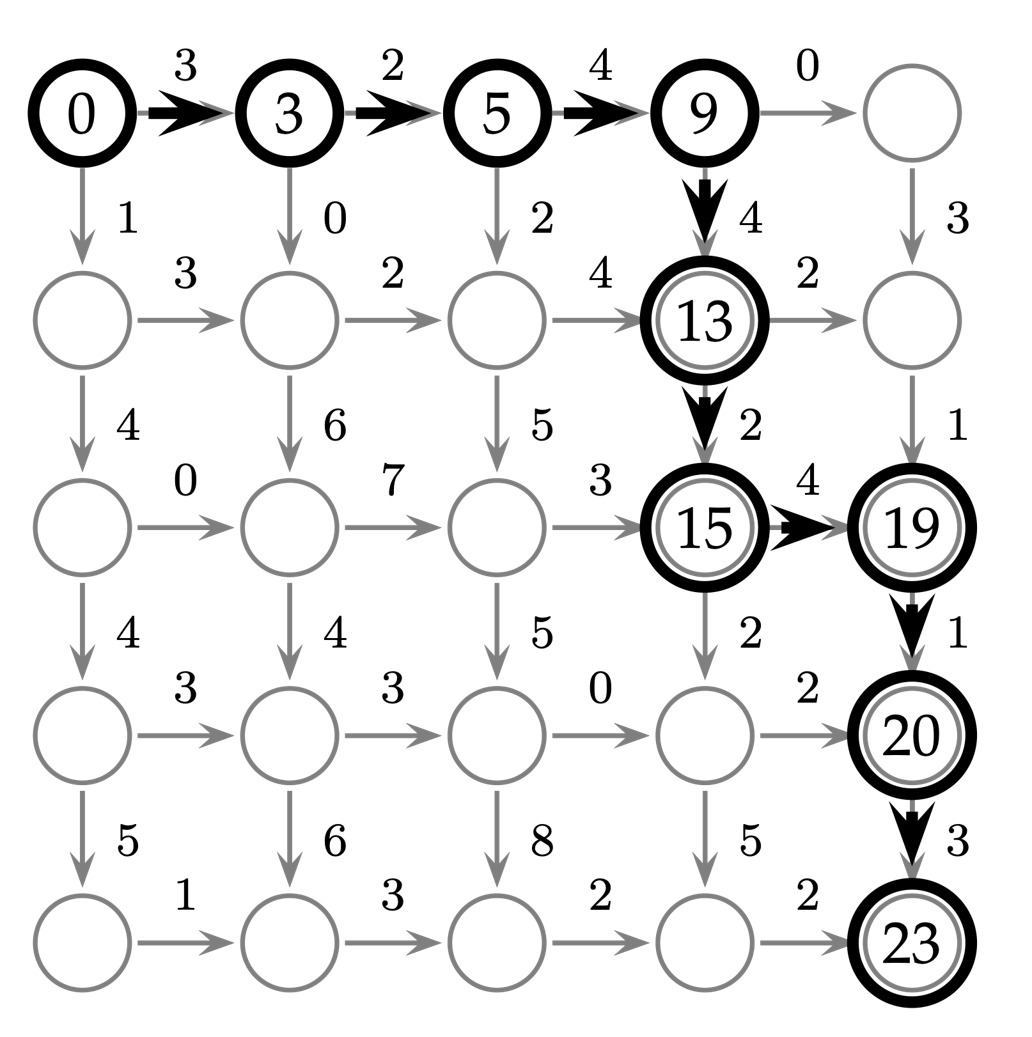
\includegraphics[width=\textwidth]{Manhattan2.png}
\end{column}
\begin{column}{0.5\textwidth}
\centering
Find the maximum-weight path from top-left to bottom-right\\
$\Downarrow$\\
Recurrence:
\[
s_{i,j} = \max\begin{cases}
s_{i-1,j} + w(\text{vertical}) \\
s_{i,j-1} + w(\text{horizontal})
\end{cases}
\]
\end{column}
\end{columns}
\end{frame}

\begin{frame}{General DP Strategy}
\begin{enumerate}
\item Turn the problem into a path-finding problem in a grid
\item Define a recurrence: value of cell $(i,j)$ depends only on a few previous cells
\item Fill table row-by-row (or column-by-column)
\item Trace back to recover the actual alignment
\end{enumerate}
\end{frame}

%------------------------------------------------
\subsection{Types of Sequence Alignment}
\begin{frame}
	\frametitle{Global, Local, Multiple}
	%	\framesubtitle{E.coli reference genome}
	
	\begin{figure}
		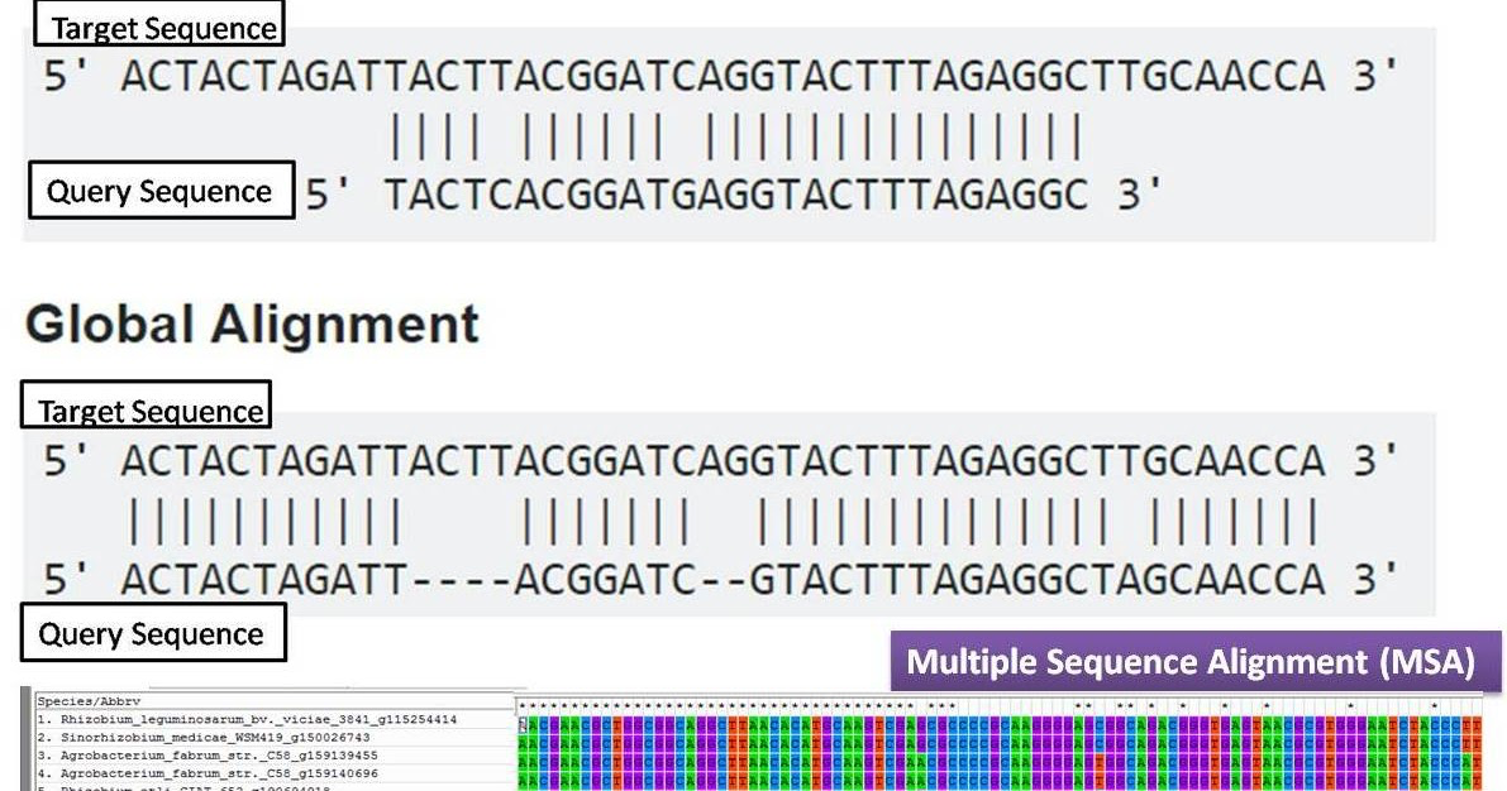
\includegraphics[width=0.8\linewidth]{global_local_multiple.png}
		\caption{Comparison between the kinds of alignment}
	\end{figure}
	
\end{frame}

%------------------------------------------------

\subsection{Global Alignment - Needleman-Wunsch}
\begin{frame}{Needleman-Wunsch (1970) - Global Alignment}
Recurrence (simplified scoring: match +1, mismatch/gap -1):
\[
F(i,j)=\max\begin{cases}
F(i-1,j-1) + s(A_i,B_j) & \text{diagonal (match/mismatch)}\\
F(i-1,j) - d         & \text{vertical (gap in B)}\\
F(i,j-1) - d         & \text{horizontal (gap in A)}
\end{cases}
\]
\end{frame}

%------------------------------------

\begin{frame}{Needleman-Wunsch Example}
\centering
\bfseries Scoring: match = +1, \quad mismatch = -1, \quad gap = -1

\bigskip
\begin{table}
\centering
\small
\begin{tabular}{c||c|cccccccc}
     & -- & A     & C     & T     & G     & A     & T     & C     & A \\
\hline
--   & \textcolor{red}{0} & -1 & -2 & -3 & -4 & -5 & -6 & -7 & -8 \\
A    & -1 & \alert{1} & \alert{0}  & -1 & -2 & -3 & -4 & -5 & -6 \\
T    & -2 & 0  & 0  & \alert{1} & 0  & -1 & -2 & -3 & -4 \\
G    & -3 & -1 & -1 & 0  & \alert{2} & 1  & 0  & -1 & -2 \\
A    & -4 & -2 & -2 & -1 & 1  & \alert{3} & 2  & 1  & 0  \\
T    & -5 & -3 & -3 & -1 & 0  & 2  & \alert{4} & 3  & 2  \\
C    & -6 & -4 & -3 & -2 & -1 & 1  & 3  & \alert{5} & 4  \\
A    & -7 & -5 & -4 & -3 & -2 & 0  & 2  & 4  & \alert{6} \\
\end{tabular}
\end{table}

\bigskip
\alert{Final score = 6} $\Rightarrow$ very good global alignment

\bigskip
\footnotesize
\begin{itemize}
\item \textcolor{red}{Red 0} = starting point (empty alignment)
\end{itemize}
\end{frame}

%------------------------------------------------

\subsection{Local Alignment - Smith-Waterman}
\begin{frame}{Smith-Waterman (1981) - Local Alignment}
Same three choices, but we are allowed to start fresh:
\[
H(i,j)=\max\begin{cases}
0 \\
H(i-1,j-1) + s(A_i,B_j) \\
H(i-1,j) - d \\
H(i,j-1) - d
\end{cases}
\]
\begin{itemize}
\item 0 means "start a new alignment here"
\item Optimal local alignment = maximum value in the entire matrix
\item Trace back from that maximum until reaching 0
\end{itemize}
\end{frame}


%------------------------------------------------

\begin{frame}
	\frametitle{Global vs. Local}
	
	\begin{figure}
		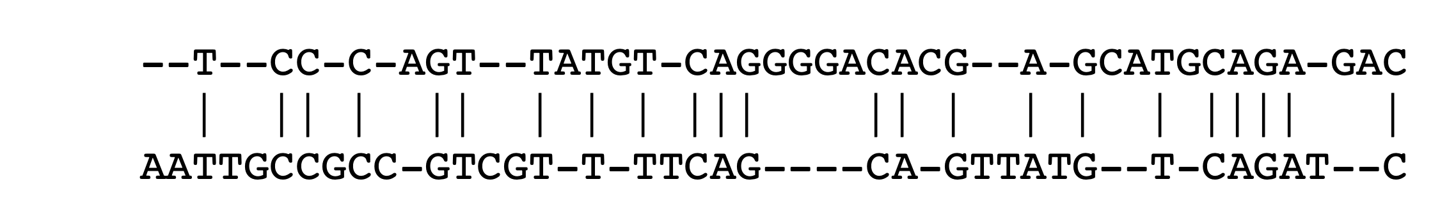
\includegraphics[width=0.9\linewidth]{glob_example.png}
		\caption{Global alignment example}
	\end{figure}
	
	\begin{figure}
		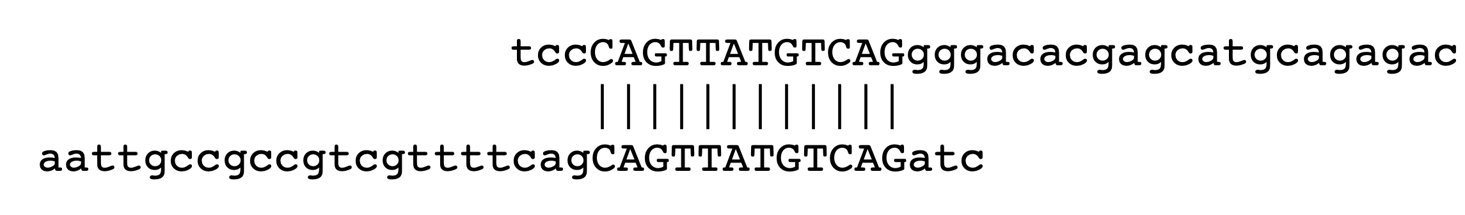
\includegraphics[width=0.9\linewidth]{loc_example.png}
		\caption{Local alignment example}
	\end{figure}
	
\end{frame}

\begin{frame}
	\frametitle{Global vs. Local}
	
	\begin{figure}
		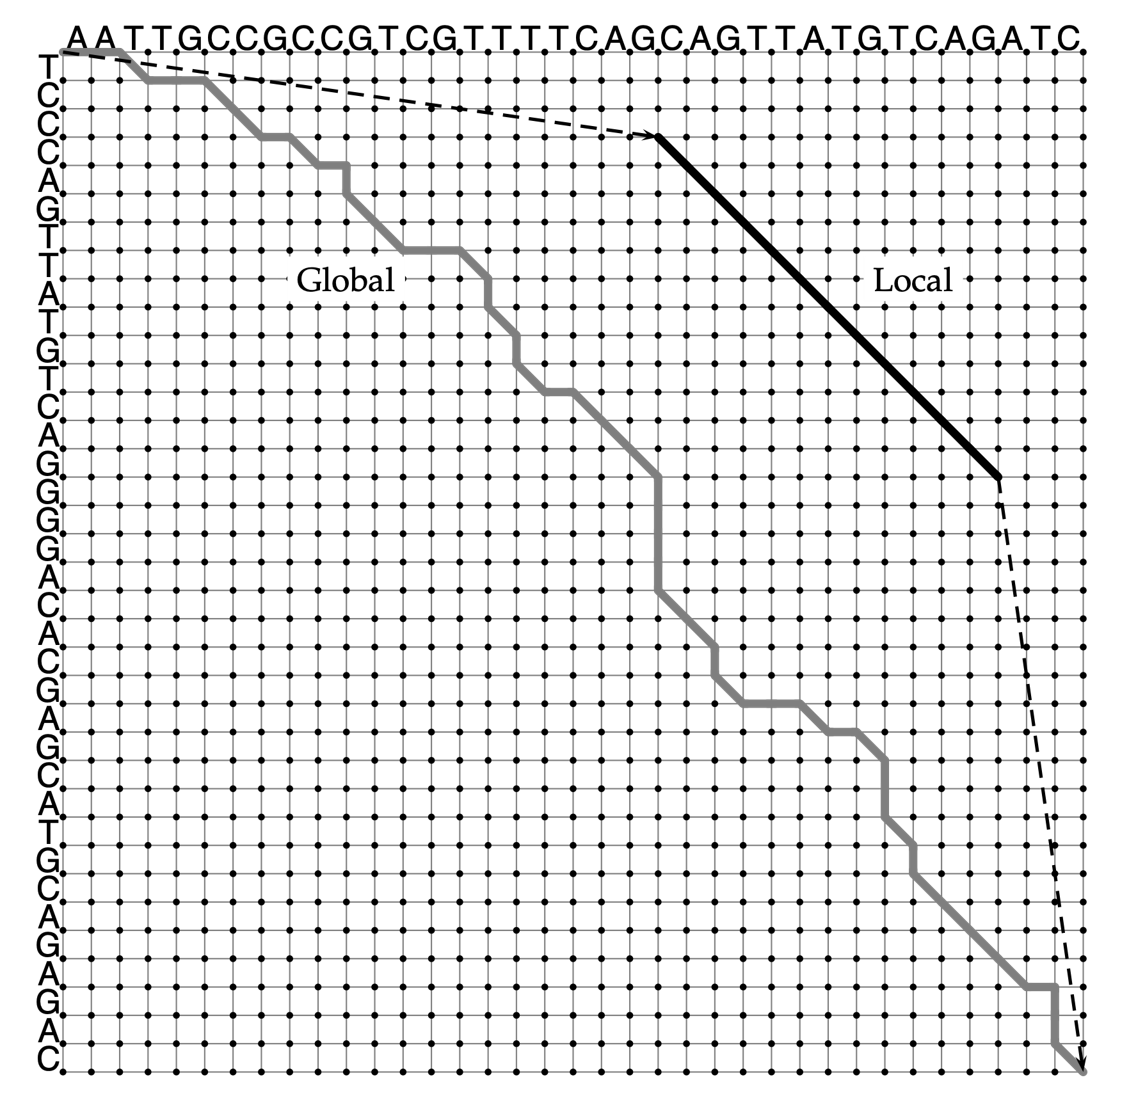
\includegraphics[width=0.5\linewidth]{glob_vs_loc_table.png}
		\caption{Comparison between the target on table}
	\end{figure}
	
\end{frame}


%------------------------------------------------
\subsection{Affine Gaps (Practical Improvement)}
\begin{frame}{Affine Gap Penalties}
Real gaps are usually long $\to$ opening a gap is more expensive than extending it.

$\Rightarrow$ Use three matrices (Gotoh 1982):
\begin{itemize}
\item $M(i,j)$ - best alignment ending with match/mismatch
\item $I_x(i,j)$ - best ending with gap in sequence x
\item $I_y(i,j)$ - best ending with gap in sequence y
\end{itemize}
Widely used in BLAST, BWA, Bowtie2, etc.
\end{frame}

%------------------------------------------------

\section{Why Pure DP is Too Slow for Read Alignment}
\begin{frame}{Complexity Problem}
\begin{itemize}
\item Needleman-Wunsch / Smith-Waterman: $O(mn)$ time and space
\item $m$ = read length (~100), $n$ = reference length (~$3\times10^{9}$)
\item Trying every position $\to$ ~$3\times10^{11}$ cell computations per read
\item Even at $10^{9}$ cells/sec $\to$ hours per read $\to$ impossible
\end{itemize}
\bigskip
\alert{Conclusion}: We cannot afford full DP for every read and every position.
\end{frame}

%------------------------------------------------


\begin{frame}
	\frametitle{Triple Sequence Alignment}
	\framesubtitle{Example}
	
	\begin{figure}
		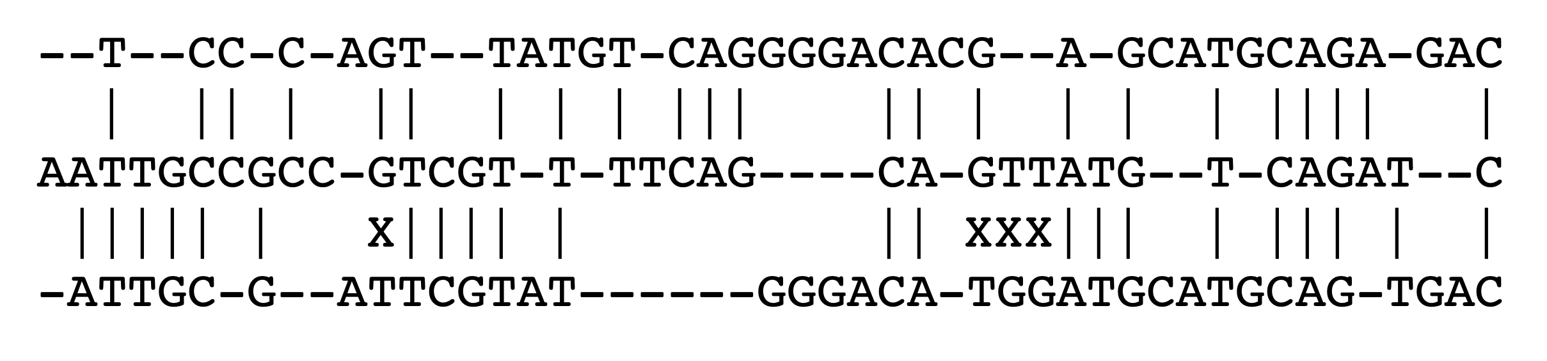
\includegraphics[width=0.8\linewidth]{triple_align.png}
		\caption{Triple alignment example}
	\end{figure}
	
\end{frame}

\begin{frame}
	\frametitle{Triple Sequence Alignment}
	\framesubtitle{Policy}
	
	\begin{figure}
		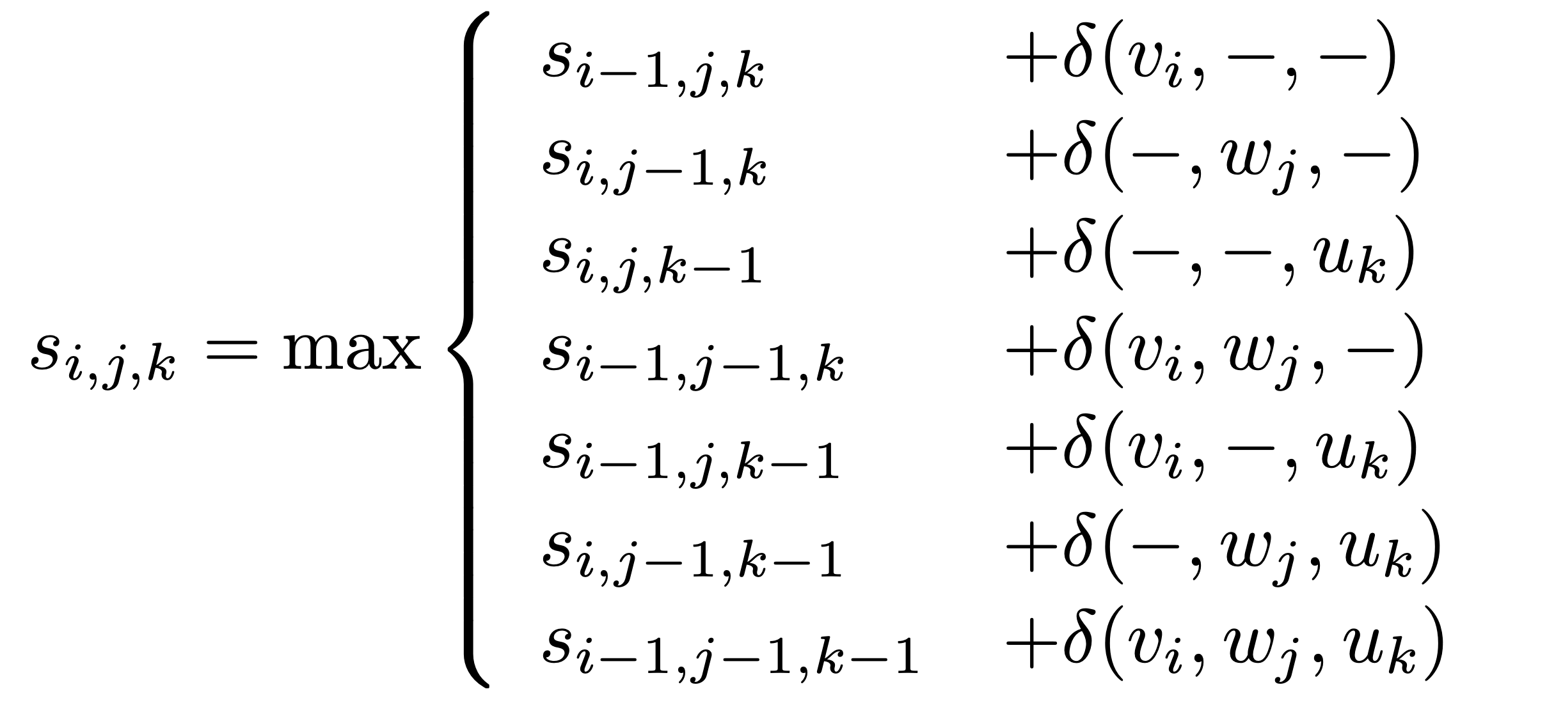
\includegraphics[width=0.75\linewidth]{triple_policy.png}
	\end{figure}
	
\end{frame}


\begin{frame}
	\frametitle{Triple Sequence Alignment}
	\framesubtitle{3-dimensional DP table}
	
	\begin{columns}[T]
		\begin{column}{0.4\textwidth}
			\centering
			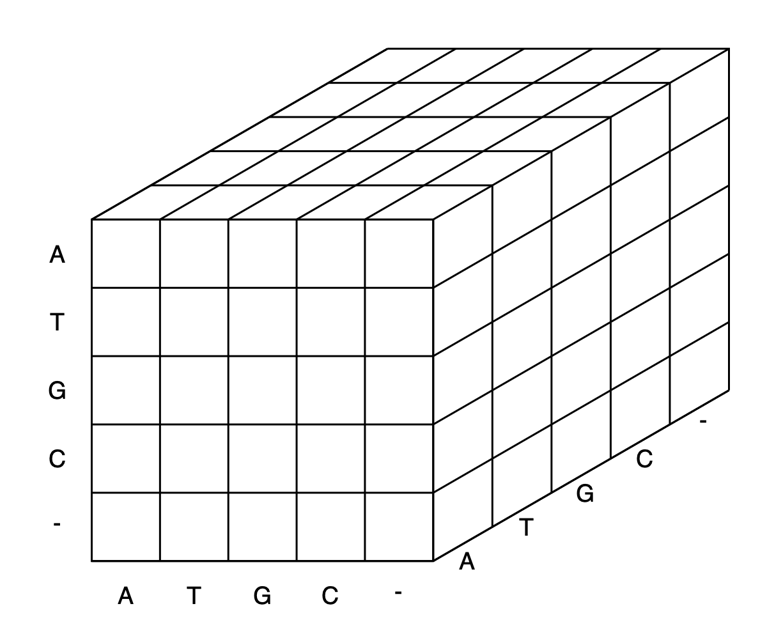
\includegraphics[width=\linewidth]{triple_cube.png}
		\end{column}
		
		\begin{column}{0.55\textwidth}
			\centering
			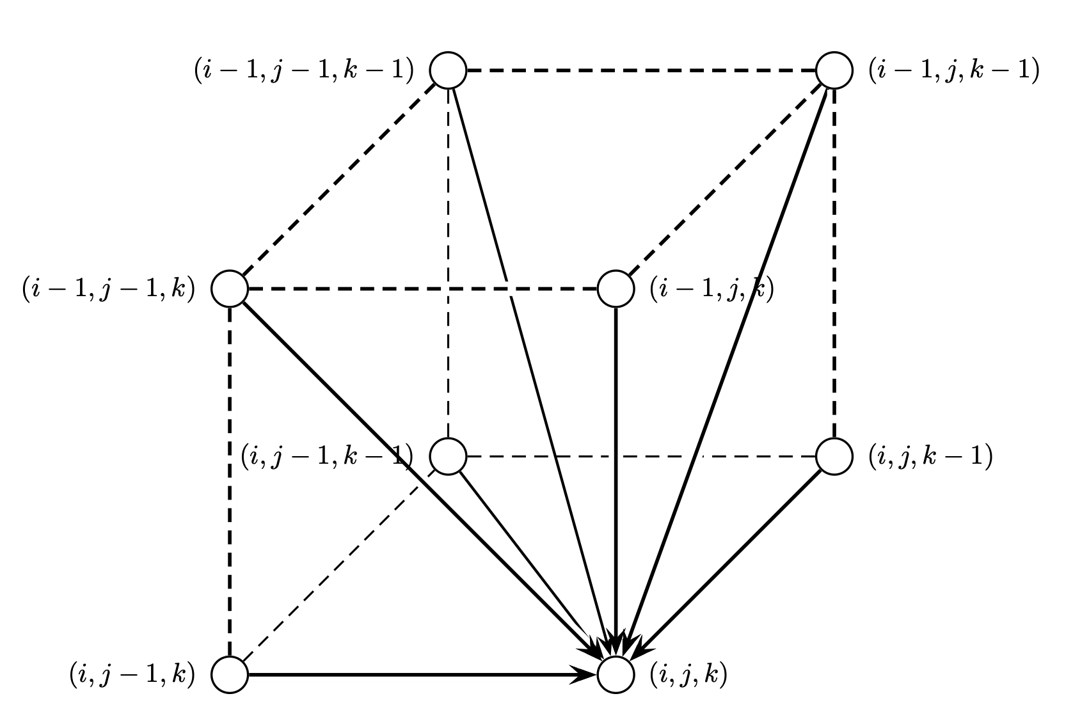
\includegraphics[width=\linewidth]{triple_corners.png}
		\end{column}
	\end{columns}
	
\end{frame}

%------------------------------------------------

\begin{frame}{Summary \& Transition}
\begin{block}{What we learned}
\begin{itemize}
\item Pairwise alignment $\to$ solved elegantly with DP
\item Global (Needleman-Wunsch) and local (Smith-Waterman)
\item Affine gaps make scoring biologically realistic
\end{itemize}
\end{block}
\bigskip
\begin{block}{But}
Pure DP is far \alert{too slow} for millions of reads against huge genomes.
\end{block}
\bigskip
\end{frame}

%------------------------------------------------
%------------------------------------------------
%------------------------------------------------
%------------------------------------------------

\section{Burrows-Wheeler Transform \& FM-Index}

\begin{frame}
\frametitle{Why the Burrows-Wheeler Transform (BWT)?}
\begin{block}{Real-world impact}
\begin{itemize}
\item Illumina NovaSeq: $>$ 3 terabases of DNA per day
\item Human genome index must fit in RAM and answer queries in microseconds
\end{itemize}
\end{block}
\bigskip
\alert{BWT powers nearly every modern short-read aligner:}
\begin{itemize}
\item Bowtie / Bowtie2 \quad BWA (MEM \& ALN) \quad minimap2 \quad SNAP \quad GEM \quad \dots
\end{itemize}
$\Rightarrow$ The single most important data structure in bioinformatics today
\end{frame}


%==============================================================================
\subsection{BWT Construction Example}
%==============================================================================
\begin{frame}
\frametitle{BWT Construction – ``panama\$'' Example}
\texttt{S = panama\$} \quad (\$ is smallest sentinel)

\begin{center}
\small
\begin{tabular}{r|l|l|c}
\# & Rotation         & Sorted rotation     & BWT \\ \hline
0  & panama\$         & \alert{\$panama}    & \alert{a} \\
1  & anama\$p         & a\$panam            & m \\
2  & nama\$pa         & ama\$pan            & n \\
3  & ama\$pan         & \alert{anama\$p}    & \alert{p} \\
4  & ma\$pana         & ma\$pana            & a \\
5  & a\$panam         & \alert{nama\$pa}    & \alert{a} \\
6  & \$panama         & panama\$            & \$ \\
\end{tabular}
\end{center}
$\Rightarrow$ \alert{BWT = amnpaa\$}
\end{frame}

%---------------------------------------------

\begin{frame}
\frametitle{The Full BWT Matrix with Ranks (LF Mapping)}

\texttt{BWT = amnpaa\$}

\bigskip
\scalebox{0.84}{
\begin{tabular}{c|c|c|c|c}
i & F (sorted)     & L[i] & Rank in L    & Rank in F $\to$ LF(i) \\ \hline
0 & \$panama       & a    & a$^{1}$      & a$^{1}$ $\to$ 1 \\
1 & a\$panam       & m    & m$^{1}$      & m$^{1}$ $\to$ 4 \\
2 & ama\$pan       & n    & n$^{1}$      & n$^{1}$ $\to$ 5 \\
3 & anama\$p       & p    & p$^{1}$      & p$^{1}$ $\to$ 6 \\
4 & ma\$pana       & a    & a$^{2}$      & a$^{2}$ $\to$ 2 \\
5 & nama\$pa       & a    & a$^{3}$      & a$^{3}$ $\to$ 3 \\
6 & panama\$       & \$   & \$$^{1}$      & \$$^{1}$ $\to$ 0 \\
\end{tabular}
}

\bigskip
alert{LF rule:} $k$-th $c$ in L $\to$ $k$-th $c$ in F
\end{frame}

%-----------------------------------------------

\begin{frame}
\frametitle{FM-Index: What We Store in Practice}
\begin{minipage}{0.58\linewidth}
\textbf{C[c]} = count of chars $<$ c
\begin{itemize}
\item C[\$]=0, C[a]=1, C[m]=4, C[n]=5, C[p]=6
\end{itemize}
\end{minipage}
\begin{minipage}{0.4\linewidth}
\textbf{Occ(c,i)} = occurrences of $c$ in BWT[0..i]
\end{minipage}

\bigskip
\alert{LF(i) = C[BWT[i]] + \text{Occ}(BWT[i], i-1)}

$\Rightarrow$ Human genome index \(\approx 3\text{--}5\ \mathrm{GB}\)
\end{frame}




%------------------------------------------------

\begin{frame}
    \frametitle{Constructing BWT from Suffix Array}

    \begin{block}{Python Code}
    {\ttfamily
    def compute\_bwt(s, sa):\newline
    \quad bwt = []\newline
    \quad for p in sa:\newline
    \quad\quad if p == 0:\newline
    \quad\quad\quad bwt.append('\$')\newline
    \quad\quad else:\newline
    \quad\quad\quad bwt.append(s[p-1])\newline
    \quad return ''.join(bwt)
    }
    \end{block}

    \begin{alertblock}{Caveat}
        Constructing the full suffix array still costs $O(n\log n)$ time 
        and $O(n)$ extra space $\Rightarrow$ this removes the memory benefits of the BWT!
    \end{alertblock}

\end{frame}


%------------------------------------------------
\begin{frame}
	\frametitle{The Crucial Property: Last-to-First (LF) Mapping}
	
	\begin{center}
		\begin{tabular}{c|c|c}
			Index $i$ & $L[i]$ (BWT) & $F[i]$ (first column) \\
			\hline
			0 & t & \$ \\
			1 & t & a \\
			2 & t & a \\
			3 & t & a \\
			4 & \$ & c \\
			5 & a & t \\
			6 & a & t \\
			7 & a & t \\
			8 & c & t \\
		\end{tabular}
	\end{center}
	
	\bigskip
	\alert{LF mapping rule:}
	If $L[i] = c$ is the $k$-th occurrence of $c$ in the BWT (column $L$),  
	then $\text{LF}(i)$ is the row where the $k$-th occurrence of $c$ appears in column $F$.
	
	\smallskip
	$\Rightarrow$ Following LF repeatedly walks \alert{backwards} through the original string!
\end{frame}

%------------------------------------------------
\begin{frame}[fragile]
	\frametitle{Decoding the Original String using LF Mapping}
	
	
	\begin{block}{Python code}
	{\ttfamily
		def decode\_bwt(bwt, LF):\\
		\quad n = len(bwt)\\
		\quad r = 0 \quad \quad \quad \quad \quad \quad \quad \quad \# start at row containing \$\\
		\quad s = ['\$']\\
		\quad while len(s) < n:\\
		\quad \quad s.append(bwt[r]) \quad \quad \# prepend the previous character\\
		\quad \quad r = LF[r] \quad \quad \quad \quad \quad \# go to previous position\\
		\quad return ''.join(reversed(s))
	}
	\end{block}
	
	\bigskip
	\alert{Result:} Starting from the \$ row and repeatedly applying LF reconstructs the original text in reverse.
\end{frame}

%------------------------------------------------
\begin{frame}
	\frametitle{LF Mapping in Practice – C and Occ arrays}
	
	We don’t store the full LF array (would cost $O(n)$ space).  
	Instead we use two small tables:
	
	\begin{itemize}
		\item $C[c]$ = number of characters \alert{strictly smaller} than $c$ in the text
		\item $\text{Occ}(c,i)$ = number of occurrences of $c$ in $\text{BWT}[0..i]$
	\end{itemize}
	
	\bigskip
	Then:
	\[
	\text{LF}(i) = C[\text{BWT}[i]] + \text{Occ}(\text{BWT}[i], i-1)
	\]
	
	$\Rightarrow$ This is the core of the \alert{FM-index} (Ferragina–Manzini 2000).
\end{frame}

%------------------------------------------------
\begin{frame}
	\frametitle{FM-Index = Compressed Full-Text Index}
	
	The FM-index supports \alert{backward searching} of patterns in $O(m)$ time (often sub-linear with sampling):
	
	\begin{enumerate}
		\item Start with interval $[0, n)$
		\item For each character $c$ of the pattern \alert{from right to left}:
		\[
		\begin{aligned}
			i' &= C[c] + \text{Occ}(c, i-1) \\
			j' &= C[c] + \text{Occ}(c, j) - 1
		\end{aligned}
		\]
		\item If $i' \le j'$ $\Rightarrow$ continue, else pattern not present
	\end{enumerate}
	
	\bigskip
	This is exactly how Bowtie, BWA-MEM, etc. find seed locations fast.
\end{frame}

%-----------------------------------------------

\begin{frame}
\frametitle{Backward Search – Find ``ana'' in ``panama\$''}
Start: [0,7) \quad Pattern: a $\to$ n $\to$ a (right to left)

\bigskip
\centering
\small
\begin{tabular}{c|c|c|c}
Step & Char & Calculation                    & Interval     \\ \hline
0    & –    & –                              & [0,7)         \\ \hline
1    & a    & 1+0=1 … 1+3=4                 & alert{[1,4)}  \\
2    & n    & 5+0=5 … 5+1=6                 & alert{[5,6)}  \\
3    & a    & 1+2=3 … 1+3=4                 & alert{[3,4)} Success \\
\end{tabular}
\normalsize

\bigskip
\alert{``ana'' occurs once, starting at position 2}
\end{frame}

%-----------------------------------------------

\begin{frame}
\frametitle{Backward Search – Visualizing Step 1 (final ``a'')}
Current interval [0,7) $\rightarrow$ looking for preceding \alert{a}

\begin{center}
\small
\begin{tabular}{c|c|c}
i & BWT[i] & F row \\
0 & \alert{a} & \$panama \\
1 & m         & a\$panam $\rightarrow$ a$^{1}$ \\
2 & n         & ama\$pan $\rightarrow$ a$^{2}$ \\
3 & p         & anama\$p $\rightarrow$ a$^{3}$ \\
4 & \alert{a} & ma\$pana \\
5 & \alert{a} & nama\$pa \\
6 & \$        & panama\$ \\
\end{tabular}
\end{center}

3× a $\rightarrow$ new interval [1,4)
\end{frame}

%=====================================================================
\begin{frame}
\frametitle{Backward Search – Step 2: Process ``n''}

Current interval: [1,4) $\to$ rows 1–3 only

We are now looking for preceding character \alert{n}

\bigskip
Only row 2 has BWT[2] = n in current range $\to$ its preceding char (via LF) is n

\bigskip
The 1st `n' in F is at row 5 $\to$ new interval becomes [5,6)
\end{frame}


%=====================================================================
\begin{frame}
\frametitle{Backward Search – Step 3: Process first ``a'' again}

Current interval: [5,6) $\to$ only row 5

BWT[5] = a $\to$ matches our pattern `a'

$\to$ maps to row 3 (3rd `a' in F)

\bigskip
Final interval [3,4) $\to$ exact match found!

\bigskip
\alert{Conclusion:} ``ana'' occurs once, starting at position 2 in ``panama\$''
\end{frame}

%------------------------------------------------
\subsection{Summary}

\begin{frame}
	\frametitle{Summary – Why BWT is Perfect for Short-Read Alignment}
	
	\begin{itemize}
		\item Reversible transformation
		\item Highly compressible (runs of identical characters)
		\item Enables \alert{exact} backward search in $O(m)$ time using only $O(n)$ bits
		\item With sampling $\Rightarrow$ locate occurrences in constant time
		\item Whole human genome index fits in \alert{$\leq 4$ GB} RAM
		\item Used by virtually every modern short-read aligner (Bowtie, BWA, etc.)
	\end{itemize}
	
	\bigskip
	\alert{Next step:} Seed-and-extend using these exact matches $\rightarrow$ fast, sensitive alignment.
\end{frame}

%------------------------------------------------

\begin{frame}{Why is Seed \& Extend Necessary?}
    \begin{itemize}
        \item A full exact BWT search works well only when the read has \textbf{no errors}.
        \item Real sequencing data contains:
        \begin{itemize}
            \item Substitutions
            \item Insertions and deletions
            \item PCR/sequencing errors
        \end{itemize}
        \item Supporting errors directly inside the BWT search is expensive.
        \item \textbf{Solution:} Modern aligners index the genome but search only short exact (or near-exact) \textbf{seeds}.
    \end{itemize}

    \begin{block}{Key Idea}
        Instead of aligning the whole read, find a reliable seed quickly,
        and then extend it locally to reconstruct the full alignment.
    \end{block}

    \begin{itemize}
        \item This reduces the search space by orders of magnitude.
        \item Makes BWT-based alignment practical, fast, and scalable.
    \end{itemize}
\end{frame}

%------------------------------------------------


\begin{frame}{Full Alignment vs. Seed \& Extend}
    \begin{columns}
        \begin{column}{0.48\textwidth}
            \textbf{Full Alignment (DP or full BWT search)}
            \begin{itemize}
                \item Attempts to align the entire read at once.
                \item Expensive in both time and memory.
                \item Error tolerance requires exploring many paths.
                \item Not scalable for billions of bases.
            \end{itemize}
        \end{column}

        \begin{column}{0.48\textwidth}
            \textbf{Seed \& Extend}
            \begin{itemize}
                \item Search only short seeds in the index.
                \item Very fast FM-index exact matching on seeds.
                \item Extension uses a small DP or local BWT search.
                \item Scales to whole human genome efficiently.
            \end{itemize}
        \end{column}
    \end{columns}

    \begin{block}{Conclusion}
        Seed \& Extend combines:
        \begin{itemize}
            \item \textbf{Speed} from FM-index seed lookup, and
            \item \textbf{Accuracy} from local DP extension.
        \end{itemize}
        This is why all modern short-read aligners use it.
    \end{block}
\end{frame}

%------------------------------------------------

\begin{frame}
	\frametitle{Contributors}
	
	\begin{center}
		\textbf{Sina Beyrami}\\[4pt]
		\textbf{Sina Daneshgar}
	\end{center}
	
\end{frame}

\section{References}

\begin{frame}
	\frametitle{References}
	\footnotesize
	\begin{itemize}
		
		\item \textbf{Istrail, S., Pevzner, P.} \textit{An Introduction to Bioinformatics Algorithms}.
		
		\item \textbf{Needleman and Wunsch} (1970) \href {https://pubmed.ncbi.nlm.nih.gov/5420325/}{\textit{A general method applicable to the search for similarities in the amino acid sequence of two proteins}}
		
		\item \textbf{Smith and Waterman} (1981) \href{https://pubmed.ncbi.nlm.nih.gov/7265238/}{\textit{Identification of common molecular subsequences}}
		
		\item \textbf{Ugene} \href{https://ugene.net/alignment-of-short-reads/}{Alignment of Short Reads} 
		
		\item \textbf{Wikipedia}
		
		\item \textbf{Sven Rahmann} (2021).  
		\href{https://www.rahmannlab.de/lehre/alsa21/02-5-bwt.pdf}{\textit{The Burrows-Wheeler Transform (BWT) – Algorithms for Sequence Analysis}}.
		
		\item \textbf{Burrows M., Wheeler D. J.} (1994).  
		\href{https://www.cs.jhu.edu/~langmea/resources/burrows_wheeler.pdf}{\textit{A block-sorting lossless data compression algorithm}}.  
		
		\item \textbf{Ferragina P., Manzini G.} (2000).  
		\textit{Opportunistic data structures with applications}.  
		
		\item \textbf{Simpson J. T., Durbin R.} (2010).  
		\textit{Efficient construction of an assembly string graph using the FM-index}.
		
		\item \textbf{Langmead B., Trapnell C., Pop M., Salzberg S. L.} (2009).  
		\textit{Ultrafast and memory-efficient alignment of short DNA sequences to the human 	genome}.  
		
		\item \textbf{Li H., Durbin R.} (2009).  
		\textit{Fast and accurate short read alignment with Burrows-Wheeler transform}. 
		
	\end{itemize}
	
\end{frame}



\end{document} 